%% Technical Report for the work on the AI-DSL over 2024

\documentclass[]{report}
\usepackage{url}
\usepackage{minted}
\usepackage[textsize=footnotesize]{todonotes}
\newcommand{\kabir}[2][]{\todo[color=yellow,author=kabir, #1]{#2}}
\newcommand{\nil}[2][]{\todo[color=purple,author=nil, #1]{#2}}
\usepackage[hyperindex,breaklinks]{hyperref}
\usepackage{breakurl}
\usepackage{listings}
\lstset{basicstyle=\ttfamily\footnotesize,breaklines=false,frame=single}
\usepackage{float}
\restylefloat{table}
\usepackage{longtable}
\usepackage{graphicx}
\usepackage[font=small,labelfont=bf]{caption}
\usepackage[skip=0pt]{subcaption}
\usepackage{circledsteps}
\usepackage{bussproofs}

%% New commands
%% \newcommand{\mettainline[1]}{\mintinline{scheme}{#1}}

\begin{document}

\title{AI-DSL Technical Report 2024}
\author{Nil Geisweiller}
\maketitle

\begin{abstract}
\end{abstract}

\tableofcontents

\chapter{Introduction}

During the middle of 2023 it became apparent that MeTTa~\cite{MeTTa}
could soon be used instead of Idris~\cite{Idris} for program
synthesis.  Around the end of 2023 a general purpose
chainer~\cite{Chaining} was developed and improved throughout 2024 and
we thus began experimenting with it to synthesize AI service
compositions.  In this document we will go over the work that was done
in order to accomplished such a feat.  It can be summarized as
follows:
\begin{itemize}
\item Develop and improve a general purpose chainer in MeTTa
  supporting backward, forward and in fact \emph{omniward} chaining
  and can handle dependent types.
\item Develop a SingularityNET Market Place crawler to gather
  information about AI services and convert that information into
  MeTTa specifications.
\item Extensively experiment with AI service composition using the
  aforementioned chainer.  Various AI service composition
  representations (including lambda abstraction and combinatory logic)
  were explored, as well as the tractability of the corresponding
  synthesis processes.
\item Prototype an AI-DSL ontology in MeTTa.
\item Implement a MeTTa to DOT converter to graphically display
  synthesized AI service compositions.
\end{itemize}
At the end of this process we finally managed to efficiently
synthesize the English to Chinese Song test case described
in~\cite{AIDSLService2023} (an add-on to the technical report of
2022~\cite{AIDSLReport2022}).  By itself this is of course very
promising.  It should be mentioned though that, in order to make the
synthesis tractable, only the services involved in that composition
were considered in the knowledge base fed to the chainer.  Attempting
to perform such synthesis while considering all available AI services
will be the subject of the next round of work on the AI-DSL.

\chapter{Type Driven Program Synthesis in MeTTa}
\label{chap:chainers}
In this chapter we will explain how program synthesis can be done in
MeTTa and go over the various backward chainers we have prototyped
during 2023 and 2024.  This will come handy for
Chapter~\ref{chap:xpaicompo} which goes over a number of experiments
on AI service compositions based on these chainers.  Why backward
chaining, you may ask?  Because it allows to go from theorems to
axioms.  In the context of AI service composition, a theorem would be
the formal specification of an overall AI service composition, such
as\\

\emph{Turn any English song into a corresponding Chinese one}\\[0.4cm]
and the axioms would be the formal specification of every AI service
involved in the composition, such as
\begin{itemize}
\item \emph{Convert speech to text.}
\item \emph{Translate English to Chinese.}
\item \emph{Turn Audio into MIDI.}
\item $\dots$
\end{itemize}
Then the backward chainer would take the overall specification and
combine existing AI services to fulfill it altogether.  Going forward
could be useful as well but for a different type of queries, such as\\

\emph{Given all these AI services, what can you come up with by
combining them?}\\[0.4cm] and the forward chainer would combine them
to form random, albeit valid, compositions and provide their formal
specifications.  Then there is everything between forward and backward
chaining, what I like to call \emph{omni} chaining.  For instance, the
query could provide an incomplete specification of the overall
composition, alongside some AI services which should be involved, and
let the omni chainer come up with completions of such specifications
using the provided AI services.  My prototypes cover all of these
possibilities, but in this report we will only focus on backward
chaining because that is what I exclusively used for the AI-DSL work
so far.
\section{Curried Backward Chainer}
\label{sec:curriedbc}

Let us begin with the Curried Backward Chainer, the simplest of them
all.  The curried backward chainer is simple because it assumes that
there is only one way to construct terms, using unary function
application.  In this case a term can be either
\begin{itemize}
\item a constant,
\item or a term applied to a term.
\end{itemize}
A constant could represent a value such as \mintinline{scheme}{42}, or
a function like a standalone AI service such as
\mintinline{scheme}{speech2text}.  In an application, the first term
must correspond to a unary function, such as \mintinline{scheme}{foo},
and the second term must correspond to its argument, such as
\mintinline{scheme}{42}, resulting in an application such as
\mintinline{scheme}{(foo 42)}.  Emulating n-ary application can be
done by considering higher order unary functions.  For instance
\mintinline{scheme}{(+ 1 2)} can be represented in curried format by
\mintinline{scheme}{((+ 1) 2)}.  Contrary to most functional
programming languages, currying is not handled automatically in MeTTa,
thus a non-curried version of \mintinline{scheme}{+} would be typed
\begin{minted}{scheme}
  (-> Number Number Number)
\end{minted}
while a curried version would be typed
\begin{minted}{scheme}
  (-> Number (-> Number Number))
\end{minted}
In the curried backward chainer, all functions are assumed to be unary
and that is how currying is handled.  As per the Curry-Howard
correspondence, functions on the programming side correspond to
inference rules on the logical side, so our curried backward chainer
can also handle synthesizing proofs, not just programs.  The AI-DSL
actually uses both sides at the same time producing AI service
compositions containing programs and proofs.  Why on earth would we
want that is explained in detail in Chapter~\ref{chap:xpaicompo}.\\

The MeTTa implementation of the curried backward chainer can be found
in~\cite{CurriedBackwardChainer} is given in full below\pagebreak
\begin{minted}{scheme}
;; Curried Backward Chainer type signature
(: bc (-> $a                            ; Knowledge base space
          Nat                           ; Maximum depth
          $b                            ; Query
          $b))                          ; Result

;; Base case
(= (bc $kb $_ (: $prf $thrm))
   (match $kb (: $prf $thrm) (: $prf $thrm)))

;; Recursive step
;; Unary proof application
(= (bc $kb (S $k) (: ($prfabs $prfarg) $thrm))
   (let* (;; Recursive call on function
          ((: $prfabs (-> $prms $thrm))
           (bc $kb $k (: $prfabs (-> $prms $thrm))))
          ;; Recursive call on argument
          ((: $prfarg $prms)
           (bc $kb $k (: $prfarg $prms))))
     ;; Query with holes filled
     (: ($prfabs $prfarg) $thrm)))
\end{minted}
Let us walk over that code.
\begin{enumerate}
\item The type signature takes
  \begin{itemize}
  \item A knowledge base containing the axioms, which can in fact be
    viewed as the rewrite rules as well.  In a way the knowledge base
    contains the description of the logic the backward chainer is
    going to operate on.
  \item A maximum depth corresponding to the maximum depth of the
    syntax tree that the backward chainer is allowed to produce.
  \item A query of the form
    \begin{minted}{scheme}
      (: TERM TYPE)
    \end{minted}
    indicating that \mintinline{scheme}{TERM} is of type
    \mintinline{scheme}{TYPE}.  The query may contains free variables
    representing holes that the backward chainer must fill.  For
    instance if the query is
    \begin{minted}{scheme}
      (: $prg (-> Number String))
    \end{minted}
    there is one big hole, \mintinline{scheme}{$prg}, in place of the
    term, indicating that the backward chainer must find a program
    with the type signature
    \begin{minted}{scheme}
      (-> Number String)
    \end{minted}
    The same backward chainer can be used to infer a type if the hole is
    placed on type.  For instance the query
    \begin{minted}{scheme}
      (: (foo 42) $type)
    \end{minted}
    indicates that the backward chainer must infer the type of
    \mintinline{scheme}{(foo 42)}.  Holes can be placed anywhere and
    at any depth across the term and the type of the query, such as
    \begin{minted}{scheme}
      (: (+ $val) (-> $input Number))
    \end{minted}
    and the backward chainer must attempt to fill the holes
    regardless.  Each result returned will be the query itself with
    the holes filled.  If more than one result exists then the
    backward chainer will return a superposition of results.
  \end{itemize}
\item The base case
  \begin{minted}{scheme}
    (match $kb (: $prf $thrm) (: $prf $thrm)))
  \end{minted}
  is simply a match query over the knowledge base. If the query is an
  axiom, then it returns it.  If it matches several axioms, then it
  returns a superposition of all matches.
\item The recursive step occurs if the query is of the form
  \begin{minted}{scheme}
    (: ($prfabs $prfarg) $thrm)
  \end{minted}
  corresponding to a unary application, and the depth is greater than
  zero, enforced by having to match the depth argument
  \mintinline{scheme}{(S $k)}.  If the backward chainer enters that
  call, then it breaks up the query into two subqueries:
  \begin{enumerate}
  \item one to discover \mintinline{scheme}{$prfabs}, the function,
  \item the other to discover \mintinline{scheme}{$prfarg}, the
    argument.
  \end{enumerate}
  \mintinline{scheme}{$prfabs} stands for \emph{proof abstraction},
  reflecting the idea that it is a function that takes a proof in
  input and outputs a proof, merely corresponding to a regular
  function on the programming side of the Curry-Howard isomorphism.
  And \mintinline{scheme}{$prfarg} stands for \emph{proof argument},
  reflecting the idea that it is an argument provided to a proof
  abstraction.  On the logical side of the Curry-Howard
  correspondence, you can roughly think of
  \mintinline{scheme}{$prfabs} as being an inference rule, while
  \mintinline{scheme}{$prfarg} being the proof of a premise of that
  inference rule.  I say roughly because \mintinline{scheme}{$prfabs}
  may not just be an inference rule, it can be more general than that,
  a proof function that takes in input a proof and outputs a proof, or
  \emph{proof abstraction} as I like to call it, which you can think
  as a composite inference rule.  The broken up query to discover the
  function is
  \begin{minted}{scheme}
    (bc $kb $k (: $prfabs (-> $prms $thrm)))
  \end{minted}
  ordering the backward chainer to look for a proof abstraction that,
  if given a proof of a premise, \mintinline{scheme}{$prms}, to be
  discovered as well, then it outputs a proof of
  \mintinline{scheme}{$thrm}, the conclusion.  The broken up query to
  discover the argument is
  \begin{minted}{scheme}
    (bc $kb $k (: $prfarg $prms))
  \end{minted}
  ordering the backward chainer to look for a proof of the premise
  \mintinline{scheme}{$prms}.
\end{enumerate}
One may notice that, unlike function definitions in regular functional
programming languages, the base case is not constrained by its depth.
In the base case of this MeTTa program, \mintinline{scheme}{$_} does
not mean \emph{otherwise}, it means \emph{any time}.  The
non-determinism of MeTTa allows both the base case and the recursive
step to be taken simultaneously.  The resulting effect is that a call
of \mintinline{scheme}{bc} can bottom down at any depth up to the
maximum depth, producing proof trees of any size up to the maximum
depth.  Let us now provide an example.  First, let us fill the
knowledge with a theory
\begin{minted}{scheme}
;; Knowledge base
!(bind! &kb (new-space))
!(add-atom &kb (: 42 Number))
!(add-atom &kb (: foo (-> Number String)))
!(add-atom &kb (: bar (-> String Bool)))
!(add-atom &kb (: . (-> (-> $b $c) (-> (-> $a $b) (-> $a $c)))))
\end{minted}
That theory expresses that \mintinline{scheme}{42} is a number,
provides two casting functions, one from \mintinline{scheme}{Number}
to \mintinline{scheme}{String}, called \mintinline{scheme}{foo}, and
the other one from \mintinline{scheme}{String} to
\mintinline{scheme}{Bool}, called \mintinline{scheme}{bar}.  Finally,
it provides a higher order composition operator \mintinline{scheme}{.}
also called the \emph{Bluebird} combinator in~\cite{TODO}.  Given that
theory we can now call the backward chainer with a few queries.  For
starter, let us infer the type of 42.
\begin{minted}{scheme}
;; Infer the type of 42
!(bc &kb Z (: 42 $type))
\end{minted}
which outputs
\begin{minted}{scheme}
[(: 42 Number)]
\end{minted}
Next, let us synthesize terms of type \mintinline{scheme}{String}
\begin{minted}{scheme}
;; Synthesize terms of type String
!(bc &kb (S Z) (: $prg String))
\end{minted}
which outputs
\begin{minted}{scheme}
[(: (foo 42) String)]
\end{minted}
The depth for this query must be at least 1, represented by
\mintinline{scheme}{(S Z)} as \mintinline{scheme}{Nat}, because the
term to be synthesized is a function application requiring to enter
the recursive step of \mintinline{scheme}{bc} at least once.  Finally,
let us synthesize all unary functions that outputs a Boolean value.
\begin{minted}{scheme}
;; Synthesize all functions that output a Boolean value
!(bc &kb (S (S Z)) (: $prg (-> $intput Bool)))
\end{minted}
which outputs the superposition of two solutions
\begin{minted}{scheme}
[(: ((. bar) foo) (-> Number Bool)),
 (: bar (-> String Bool))]
\end{minted}
one turning a number into a Boolean value,
\mintinline{scheme}{((. bar) foo)}, the other one turning a string
into a Boolean value, \mintinline{scheme}{bar}.\\

To help you understand what is going I have printed the trace of the
\mintinline{scheme}{bc} call of the last query.
\mintinline{scheme}{bc-bas} corresponds to the base case entry,
\mintinline{scheme}{bc-rec} corresponds to the recursive step entry.
The knowledge base argument is missing from the trace to be more
concise.  I have manually reconstructed the tree representing the
recursive calls and added some comments.  Note that the tree does not
show the distinction between non-determinism across branches and
regular functional evaluation along one branch.  I hope the trace
conveys what is going on in spite of that omission.  Obviously it
would be nice if MeTTa could offer a tool to automatically display
such trace and show such distinctions.\\
\begin{footnotesize}
\begin{minted}{scheme}
| ;; Original call, base case, succeeds (match bar)
|-(bc-bas (S (S Z)) (: $prg (-> $intput Bool)))
| ;; Original call, recursive step
|-(bc-rec (S (S Z)) (: ($prfabs#219 $prfarg#220) (-> $intput Bool)))
  | ;; First recursive call on function, base case, fails
  |-(bc-bas (S Z) (: $prfabs#219 (-> $prms#222 (-> $intput Bool))))
  | ;; First recursive call on function, recursive step
  |-(bc-rec (S Z) (: ($prfabs#730 $prfarg#731) (-> $prms#222 (-> $intput Bool))))
  | | ;; Second recursive call on function, base case, succeeds (match .)
  | |-(bc-bas Z (: $prfabs#730 (-> $prms#733 (-> $prms#222 (-> $intput Bool)))))
  | | ;; Second recursive call on argument, base case, succeeds (match bar)
  | |-(bc-bas Z (: $prfarg#731 (-> $b#1364 Bool)))
  | ;; First recursive call on argument, base case, succeeds (match foo)
  |-(bc-bas (S Z) (: $prfarg#220 (-> $intput String)))
  | ;; First recursive call on argument, recursive step
  |-(bc-rec (S Z) (: ($prfabs#2202 $prfarg#2203) (-> $intput String)))
    | ;; Second recursive call on function, base case, fails
    |-(bc-bas Z (: $prfabs#2202 (-> $prms#2205 (-> $intput String))))
\end{minted}
\end{footnotesize} Upon the second recursive call on function, entering the base case
\begin{small}
\begin{minted}{scheme}
(bc-bas Z (: $prfabs#730 (-> $prms#733 (-> $prms#222 (-> $intput Bool)))))
\end{minted}
\end{small} the successful match of the query against
\begin{small}
\begin{minted}{scheme}
(: . (-> (-> $b $c) (-> (-> $a $b) (-> $a $c))))
\end{minted}
\end{small}
creates bindings which are passed upstream to
the caller (the first recursive call on function).  As a result, by
the time the second recursive call on argument enters the base case
\begin{small}
\begin{minted}{scheme}
(bc-bas Z (: $prfarg#731 (-> $b#1364 Bool)))
\end{minted}
\end{small} the premise \mintinline{scheme}{$prms#733} has been substituted by
\mintinline{scheme}{(-> $b#1364 Bool)}.  This comes from
\mintinline{scheme}{(-> $b $c)} because \mintinline{scheme}{$c} was
unified with \mintinline{scheme}{Bool} while attempting to match
\mintinline{scheme}{(-> $intput Bool)} against
\mintinline{scheme}{(-> $a $c)}.\\

If at this point what is going on is still unclear, I recommend to run
the code, query by query, while tracing the function calls.  To that
end I have included a file~\cite{TODO}
\begin{minted}{bash}
  curry-backward-chainer-example.metta
\end{minted}
containing the code described above, wrapped in \texttt{trace!} calls.
As its name indicates \texttt{trace!} is a MeTTa primitive to trace
MeTTa code.

\section{Uncurried Backward Chainer}

It is not always convenient to manipulate curried expression, in that
case, extending the curried backward chainer to support more than
unary functions can be done by adding more entries in the backward
chainer definition.  Specifically, right below the unary proof
application recursive step
\begin{minted}{scheme}
;; Unary proof application
(= (bc $kb (S $k) (: ($prfabs $prfarg) $thrm))
   ...)
\end{minted}
one may simply add
\begin{minted}{scheme}
;; Binary proof application
(= (bc $kb (S $k) (: ($prfabs $prfarg1 $prfarg2) $thrm))
   (let* (;; Recursive call on function
          ((: $prfabs (-> $prms1 $prms2 $thrm))
           (bc $kb $k (: $prfabs (-> $prms1 $prms2 $thrm))))
          ;; Recursive call on first argument
          ((: $prfarg $prms1)
           (bc $kb $k (: $prfarg1 $prms1)))
          ;; Recursive call on second argument
          ((: $prfarg $prms2)
           (bc $kb $k (: $prfarg2 $prms2))))
     ;; Query with holes filled
     (: ($prfabs $prfarg1 $prfarg2) $thrm)))
\end{minted}
to support uncurried binary functions.  Or
\begin{minted}{scheme}
;; Ternary proof application
(= (bc $kb (S $k) (: ($prfabs $prfarg1 $prfarg2 $prfarg3) $thrm))
   (let* (;; Recursive call on function
          ((: $prfabs (-> $prms1 $prms2 $prms3 $thrm))
           (bc $kb $k (: $prfabs (-> $prms1 $prms2 $prms3 $thrm))))
          ;; Recursive call on first argument
          ((: $prfarg $prms1)
           (bc $kb $k (: $prfarg1 $prms1)))
          ;; Recursive call on second argument
          ((: $prfarg $prms2)
           (bc $kb $k (: $prfarg2 $prms2)))
          ;; Recursive call on third argument
          ((: $prfarg $prms3)
           (bc $kb $k (: $prfarg3 $prms3))))
     ;; Query with holes filled
     (: ($prfabs $prfarg1 $prfarg2 $prfarg3) $thrm)))
\end{minted}
to support uncurried ternary functions, etc.  One may write a MeTTa
macro (which is just a regular MeTTa program) to generate such code
for any given arity.  Although since the arities of the functions we
manipulate for reasoning are usually low, we have not found the need
to do that so far.

\section{Embed Inference Rules}

Another possible extension of the backward chainer is to embed its
axioms and inference rules directly in its code.  For instance the
theory given in example in Section~\ref{sec:curriedbc} we be directly
implemented as the following specialized backward chainer

\begin{minted}{scheme}
;; Base cases
(= (bc $_ (: 42 Number)) (: 42 Number))
(= (bc $_ (: foo (-> Number String))) (: foo (-> Number String)))
(= (bc $_ (: bar (-> String Bool))) (: bar (-> String Bool)))

;; Recursive step
;; Function composition
(= (bc (S $k) (: (. $prfarg1 $prfarg2) (-> $a $c)))
   (let* (;; Recursive call on first argument
          ((: $prfarg1 (-> $b $c))
           (bc $kb $k (: $prfarg1 (-> $b $c))))
          ;; Recursive call on second argument
          ((: $prfarg2 (-> $a $b))
           (bc $kb $k (: $prfarg2 (-> $a $b)))))
      (: (. $prfarg1 $prfarg2) (-> $a $c))))
\end{minted}
In this example the entire theory is embedded in the backward chainer
implementation, but one can also write a hybrid backward chainer with
some rules being generic, and some being embedded in the code.  One
advantage of embedding the theory directly in the backward chainer
implementation is that some axioms or rules can be given some special
treatments.  Examples of such implementations will be shown in
Chapter~\ref{TODO}.

\section{Dependent Types}

Simply explained, \emph{dependent types}~\cite{TODO} allow to use
values inside types.  An example of what can be done with dependent
types that is often given is a vector data structure where the size of
the vector is specified within the type itself.  Such definition may
in Idris look like
\begin{minted}{idris}
-- Vector type parameterized by element type and size
Vect : a -> Nat -> Type

-- Build a vector by repeating a given element n times
repeat : a -> (n : Nat) -> (Vect a n)
\end{minted}
Given that definition one may build the following
\begin{minted}{idris}
(repeat "abc" 42) : (Vect String 42)
\end{minted}
corresponding to a vector of 42 strings of \mintinline{idris}{"abc"}.
One can then pursue to write operators manipulating vectors allowing
consistency checking on their sizes to take place at compile time.
For instance \mintinline{idris}{append} would have the following type
signature
\begin{minted}{idris}
-- Append one vector of size n with another one of size m
append : (Vect a n) -> (Vect a m) -> (Vect a (n + m))
\end{minted}
Note that the vector size inside the output type is
\mintinline{idris}{(n + m)}.\\

As of today, dependent types are not supported by the built-in type
checker of MeTTa.  Luckily for us however, only a few modifications
need to be operated to have the backward chainer support dependent
types in MeTTa.

\subsection{Rule Format for Dependent Types}
\label{subsec:frmtdt}
First, the format of an inference rule must be changed from
\begin{minted}{scheme}
(-> PREMISE CONCLUSION)
\end{minted}
to
\begin{minted}{scheme}
(-> (: ARGUMENT PREMISE) CONCLUSION)
\end{minted}
where \mintinline{scheme}{ARGUMENT} would typically appear inside
\mintinline{scheme}{CONCLUSION}, the \emph{dependent} part of
dependent types.  An example of such inference rule would be
\begin{minted}{scheme}
(: translate
   (-> (: $src-lang NaturalLanguage) (: $dst-lang NaturalLanguage)
       (-> (: $_ (TextIn $src-lang)) (TextIn $dst-lang))))
\end{minted}
This inference rule represents an actually AI service from the
SingularityNET market place that translates a text in some source
language to an equivalent text in some destination language.  The
first two arguments of the type signature of the service are the
source and destination languages
\begin{minted}{scheme}
(: $src-lang NaturalLanguage)
(: $dst-lang NaturalLanguage)
\end{minted}
Because the argument terms, \mintinline{scheme}{$src-lang} and
\mintinline{scheme}{$dst-lang}, are specified in the type signature,
they can be passed as parameters to the other following types
\begin{minted}{scheme}
(TextIn $src-lang)
(TextIn $dst-lang)
\end{minted}
where \mintinline{scheme}{TextIn} is a parameterized type representing
a text in a given language.  One may notice the use of
\mintinline{scheme}{$_} representing a variable that is not
subsequently used to create dependencies\footnote{Please be aware that
in MeTTa \mintinline{scheme}{$_} is a regular variable and does behave
like an underscore in a functional programming language like Haskell.
Thus multiple occurrences of \mintinline{scheme}{$_} within the same
scope still will point to the same variable.}.  That is because in the
current format, unlike in Idris, specifying the argument associated to
the input of an arrow type is mandatory.  This may eventually become
optional to have more concise type signatures.  One may also notice
that the rule is a mixture of curried and uncurried arguments.  The
first two arguments are uncurried while the last one is curried.  This
is perfectly fine and comes from a convention that has been adopted in
some experiments, which is that arguments of AI services corresponding
to hyper-parameters are uncurried, while those corresponding to data
being processed are curried.  The reason for this convention is
explained in detail in Chapter~\ref{TODO}.

\subsection{Backward Chainer for Dependent Types}

With all that said, modifying the backward chainer to support
dependent types is as trivial as it may be.  The code is identical to
the backward chainers presented above but the queries must follow the
format presented in Subsection~\ref{subsec:frmtdt}.  The full
implementation for the modified curried backward chainer is given
below
\begin{minted}{scheme}
;; Dependently Typed Curried Backward Chainer type signature
(: bc (-> $a                            ; Knowledge base space
          Nat                           ; Maximum depth
          $b                            ; Query
          $b))                          ; Result

;; Base case
(= (bc $kb $_ (: $prf $thrm))
   (match $kb (: $prf $thrm) (: $prf $thrm)))

;; Recursive step
;; Unary proof application
(= (bc $kb (S $k) (: ($prfabs $prfarg) $thrm))
   (let* (;; Recursive call on function
          ((: $prfabs (-> (: $prfarg $prms) $thrm))
           (bc $kb $k (: $prfabs (-> (: $prfarg $prms) $thrm))))
          ;; Recursive call on argument
          ((: $prfarg $prms)
           (bc $kb $k (: $prfarg $prms))))
     ;; Query with holes filled
     (: ($prfabs $prfarg) $thrm)))
\end{minted}
Only two lines have changed, the query of the recursive call on
function has gone from
\begin{minted}{scheme}
(: $prfabs (-> $prms $thrm))
\end{minted}
to
\begin{minted}{scheme}
(: $prfabs (-> (: $prfarg $prms) $thrm))
\end{minted}
that is all.  An example of using such dependently typed backward
chainer to prove properties about programs can be found in~\ref{TODO}.
The chainer used for most of the AI-DSL experiments is based on it,
with the additional support for uncurried and embedded rules.  We are
almost done regarding chaining, but there is one last extension we
need to cover because some experiments were conducted with it, the
support for lambda abstraction.

\section{Lambda Abstraction}

In $\lambda$-calculus, lambda abstraction, or $\lambda$ abstraction,
is a way to construct functions.  On the proof side of the
Curry-Howard correspondence, $\lambda$ abstraction is a way to
construct proof functions, or what I like to call \emph{proof
abstractions}, a function that takes a proof in argument and outputs a
proof.  If the argument is the proof of a certain hypothesis $H$, and
the output is a proof of a conclusion $C$, then the proof abstraction
is a function that computes a way to go from a proof of $H$ to a proof
of $C$, which can be denoted with the arrow type as $H \to C$.
Function construction is the dual of function application.  Just like
function construction can be viewed as hypothesis introduction,
function application can be viewed as modus ponens.  That is, given a
body $c : C$, containing a free variable $x$ of type $H$, one can use
lambda abstraction to construct the following implication $$\lambda
x. c : H \to C$$ Likewise, applying such proof abstraction to proof $h
: H$, results in proof $$((\lambda x. c)\ h) : C$$ which, one may
note, perfectly emulates the behavior of the modus ponens rule.  Thus
one may consider that the backward chainer presented so far is
essentially a generic implementation of modus ponens.  It makes sense
therefore that one would want to support its dual operation, lambda
abstraction.  There is an alternative though, which is to use
\emph{Combinatory Logic}.  A combinator is a higher order function
that takes functions in inputs and output yet more functions.  Some
combinator set, such as S, K and I are known to be sufficiently
expressive so that one can built any function out of them.  That is
how they can represent an alternative to $\lambda$ abstraction.  Our
most successful experiments were in fact conducted with combinators
(albeit another set than S, K and I), while most of our experiments
conducted with $\lambda$ abstraction failed due to the excessive and
uncontrollable combinatorial explosion resulting from it.  The
backward chainer implementations presented so far already support
combinaroty logic, one just needs to define the set of combinators to
be used in the theory handed to the backward chainer.  For $\lambda$
abstraction it is a bit more complicated and the backward chainer
needs to be modified specifically for that purpose.  Let us show below
how.

\subsection{Backward Chaining with Lambda Abstraction}

The main idea needed to have the backward chainer support $\lambda$
abstraction is that, when going backward, unpacking a $\lambda$
abstraction must introduce knowledge in the theory about the type of
the variable previously scoped by the $\lambda$.  Formally, this can
be represented as the following inference rule
\begin{prooftree}
  \AxiomC{$\Gamma, x : s \vdash f : t$}
  \RightLabel{($\lambda$ Introduction)}
    \UnaryInfC{$\Gamma \vdash \lambda x.f : s \to t$}
\end{prooftree}
meaning that if $\lambda x.f$ is typed $s \to t$ in theory $\Gamma$,
then, as we go backward, to be able to infer the type of $f$, we need
to add information about the type of $x$ into $\Gamma$.  Indeed, as
the backward chainer keeps unpacking $f$, it will eventually meet $x$,
then query the theory about its type.  If the type is missing the
backward chainer will fail to reach all the axioms, and thus fail to
infer the type of $f$.  In other words, for $\lambda$ abstraction to
be properly supported, $x: s$ must temporarily become an axiom of the
theory as backward chaining is taking place.

Going back to MeTTa, in our backward chaining implementations the
theory is stored in a space for efficiently matching inference rules
and axioms.  So far the theory was static, only defined once before
launching the backward chainer and left unchanged while running.  To
support $\lambda$ abstraction however, we need to be able to
dynamically and locally modify such space in every non-deterministic
branches as the backward chainer unpacks $\lambda$ abstractions.
Unfortunately, MeTTa does not support locally modifying spaces, though
an issue~\cite{TODO} has been created and it will hopefully be
supported in the foreseeable future.  In the meantime we have
implemented our own data structure alongside a custom match operator
mimicking what a locally modifiable space would do.  It is not
efficient, our custom match operator is linear in complexity, but it
gives us the tools that we need to experiment with $\lambda$
abstraction, as well as any other reasoning schemes involving
dynamically modifying a theory, such as modal and contextual
reasoning, which are not presented in this document but are also of
capital importance.

\subsection{Locally Modifying Space}

Below is the code of our MeTTa implementation of a locally modifiable
space.
%% \begin{small}
\begin{minted}{scheme}
;; Define match', like match but takes a list of terms as space
(: match' (-> (List Atom) $a $a $a))
;; Base case, empty space
(= (match' Nil $pattern $rewrite) (empty))
;; Base case, match with the head
(= (match' (Cons $h $t) $p $r) (let $p $h $r))
;; Recursive step, match with the tail
(= (match' (Cons $h $t) $p $r) (match' $t $p $r))
\end{minted}
%% \end{small}
So a space is merely a list of MeTTa terms.  Once more,
non-determinism is put to use to iterate over the list while returning
the superposition of matches.  For the sake of completeness the code
of \mintinline{scheme}{List} is provided below
%% \begin{small}
\begin{minted}{scheme}
;; Define List data type and constructors
(: List (-> $a Type))
(: Nil (List $a))
(: Cons (-> $a (List $a) (List $a)))
\end{minted}
%% \end{small}

\subsection{Encoding Variables as De Bruijn Indices}

In the backward chainer, MeTTa variables take the role of holes in the
query.  In order to enable the backward chainer to manipulate
variables in the proofs and programs being synthesized while avoiding
any possible confusion with holes, proof and program variables are
encoded as De Bruijn indices.
\begin{minted}{scheme}
;; Define DeBruijn type and constructors
(: DeBruijn Type)
(: z DeBruijn)                        ; Zero
(: s (-> DeBruijn DeBruijn))          ; Successor
\end{minted}
Thus \mintinline{scheme}{z} represents the first De Bruijn index,
\mintinline{scheme}{(s z)} represents the second,
\mintinline{scheme}{(s (s z))} represents the third, and so on.  One
may notice that \mintinline{scheme}{DeBruijn} is isomorphic to
\mintinline{scheme}{Nat}
\begin{minted}{scheme}
;; Define Nat type and constructors
(: Nat Type)
(: Z Nat)
(: S (-> Nat Nat))
\end{minted}
It still needs to be provided though so that the backward chainer can
make the distinction between a natural number and a variable.

\subsection{Lambda Abstraction in MeTTa}
With all that in hand we can finally provide the full implement of the
backward chainer supporting $\lambda$ abstraction.  Let us start with
its type signature.
\begin{minted}{scheme}
;; Define Backward Chainer with Lambda Abstraction
(: bc (-> $a                            ; Knowledge base space
          (List $b)                     ; Environment
          DeBruijn                      ; De Bruijn Index
          Nat                           ; Maximum depth
          $b                            ; Query
          $b))                          ; Result
\end{minted}
Compared to the backward chainer implementations above, two extra
arguments are introduced:
\begin{itemize}
\item An environment, typed \mintinline{scheme}{(List $b)}, holding
  the dynamic part of the theory, solely dedicated to store typing
  relationships of variables dynamically introduced by the backward
  chainer as it encounters $\lambda$ abstractions.  While the
  knowledge base space still statically holds the rest of the theory.
\item A De Bruijn index, typed \mintinline{scheme}{DeBruijn}, to be
  used as variable for the next encountered $\lambda$ abstraction.
\end{itemize}
For instance, let us say the backward chainer is called on
\begin{minted}{scheme}
(bc $kb Nil z (S (S Z)) (: (\ z (+ z z)) (-> Number Number)))
\end{minted}
corresponding to a type checking query of
\mintinline{scheme}{(\ z (+ z z))},  an anonymous function which
doubles a number, against the type \mintinline{scheme}{(-> Number Number)}.
Initially, the environment is empty, \mintinline{scheme}{Nil}, meaning no
variable has been introduced so far, or equivalently, no lambda
abstraction was encountered so far.  The De Bruijn index to be
introduced next is \mintinline{scheme}{z}, matching the index in the
$\lambda$ abstraction of the query.  Subsequently, a
recursive call is crafted by the backward chainer to
\begin{enumerate}
\item unpack the $\lambda$ abstraction,
\item insert typing information about \mintinline{scheme}{z} in the
  environment, here \mintinline{scheme}{(: z Number)},
\item increment the De Bruijn index, thus \mintinline{scheme}{(s z)},
  for a future potential lambda abstraction.
\end{enumerate}
The resulting call looks like
\begin{minted}{scheme}
(bc $kb (Cons (: z Number) Nil) (s z) (S Z) (: (+ z z)) Number))
\end{minted}
At this point the backward chainer still needs to unpack
\mintinline{scheme}{(+ z z)} and go one level deeper in the
recursion to reach the axioms
\begin{minted}{scheme}
(bc $kb (Cons (: z Number) Nil) (s z) Z (: z Number))
\end{minted}
which it can, since the query \mintinline{scheme}{(: z Number)}
unifies with one the axioms in the environment, which happens to be a
singleton in this example.  The full implementation of the backward
chainer supporting $\lambda$ abstraction is given below.
\begin{small}
\begin{minted}{scheme}
;; Base cases
;; Match the knowledge base
(= (bc $kb $env $idx $_ (: $prf $thrm))
   (match $kb (: $prf $thrm) (: $prf $thrm)))
;; Match the environment
(= (bc $kb $env $idx $_ (: $prf $thrm))
   (match' $env (: $prf $thrm) (: $prf $thrm)))

;; Recursive steps
;; Proof application
(= (bc $kb $env $idx (S $k) (: ($prfabs (: $prfarg $prms)) $thrm))
   (let* (((: $prfabs (-> $prms $thrm))
           (bc $kb $env $idx $k (: $prfabs (-> $prms $thrm))))
          ((: $prfarg $prms)
           (bc $kb $env $idx $k (: $prfarg $prms))))
     (: ($prfabs (: $prfarg $prms)) $thrm)))
;; Proof abstraction
(= (bc $kb $env $idx (S $k) (: (\ $idx $prfbdy) (-> $prms $thrm)))
   (let (: $prfbdy $thrm)
     (bc $kb (Cons (: $idx $prms) $env) (s $idx) $k (: $prfbdy $thrm))
     (: (\ $idx $prfbdy) (-> $prms $thrm))))
\end{minted}
\end{small}
I am hoping that by now the mechanism is clear.  If it is not, feel
free to play with the implementation and the examples provided
in~\cite{TODO, TODO}.

We have covered everything we need to know in order to synthesize AI
services compositions in a type driven manner using MeTTa.  An obvious
prerequisite though, is to have the knowledge of AI services and their
type specifications, in the first place.  The next Chapter will look
into the problem of retrieving such information from the
SingularityNET Market Place.

\chapter{Representing the SingularityNET Market Place in MeTTa}
\label{chap:marketplace}
\section{SingularityNET and the Blockchain}
Explaining in detail how the SingularityNET Market Place works is
beyond the scope of this document, but let me nonetheless attempt to
give you a high level view of how the SingularityNET Market Place
operates on the blockchain.  We will focus on the Ethereum blockchain
because it is the one that I understand, but I believe what I am about
to say applies to the Cardano blockchain side of SingularityNET as
well.

A smart contract on the Ethereum blockchain centralizes the process of
registering organizations that want to publish services on the
SingularityNET Market Place.  You may ask, ``centralizes'', I thought
it was decentralized?  Yes, it is decentralized in the sense that the
contract is ultimately duplicated all over the Ethereum network, but
it is centralized in the sense that any modification of it will
disperse over the network until a consensus is reached, so that in the
end, there is a universal agreement on what this contract contains.
Once an organization is registered, it can register AI services via
interacting with the same smart contract.  Due to the high cost of
holding data on the Ethereum blockchain, the smart contract only holds
the minimal amount of data, such as organization identifiers, wallets,
the list of their services, etc.  More data hungry information such as
the descriptions of the services are stored in the InterPlanetary File
System (IPFS for short), a decentralized, data immutable, content
addressable storage system.  The smart contract then only needs to
point to the right IPFS addresses to retrieve the desired information.
Given the immutability of data of IPFS, once a smart contract points
to a given address, it is guarantied that the content at that address
will not change.  To change it, the smart contract must be modified to
point to another address.  Thus, all possible modification are
funneled through the smart contract.  That is not to say that the
network cannot change if the smart contract is not changed, for
instance a service provider may decide to silently shut down its
servers, but the description itself of the SingularityNET Market Place
should be immune to these external circumstances.  That is of course
assuming that both the Ethereum blockchain and the IPFS networks are
collectively given the care to operate as intended.  In particular,
for IPFS, there needs to be at least one node in the network
containing the data referenced by the SingularityNET smart contract.

\section{Crawling the SingularityNET Market Place}
\label{sec:csnmp}
The goal of this process is to gather information about all AI
services on the SingularityNET Market Place and convert that
information into a format that the backward chainer can use to
synthesize AI service compositions.

To that end, a bash script driving the SingularityNET
CLI~\cite{SNETCLI} has been implemented to crawl the SingularityNET
Market Place, see~\cite{TODO}.  First, it gathers all organizations
and their services in JSON format.  Second, it converts that into
MeTTa.  It can afford to be implemented in bash because the heavy
lifting of accessing the information inside the smart contract is
outsourced to the SingularityNET CLI, and then reading that
information in JSON format is outsourced to jq~\cite{JQ}, a
command-line JSON processor.  At the end of the process we are left
with a folder tree structure of JSON files organized by organizations
and services, and a monolithic MeTTa file containing the definitions
of all organizations, their services and their associated type
signatures.

Such MeTTa file can then be imported in a space and used to reason
about organizations and their services, and in particular for what is
our main interest here, to reason about their compositions.  One can
find examples of such monolithic dumps in MeTTa format in~\cite{TODO}.
Let us give a few snippets of such a dump for illustrative purposes.
For instance, the data type to represent an organization is defined in
MeTTa as follows:
%% \pagebreak
\begin{minted}{scheme}
;; Define Organization type
(: Organization Type)

;; Define Organization constructor
(: MkOrganization
   (->
       String ; org_name
       String ; org_id
       String ; org_type
       Description ; description
       (List Assets) ; assets
       (List Contact) ; contacts
       (List Group) ; groups
       Organization))
\end{minted}
One may immediately notice that the format is consistent with the
format of axioms and inference rules the backward chainer expects, a
collection of typing relationships.  An example of the definition of
an object of the type \mintinline{scheme}{Organization}, here
corresponding to the SingularityNET organization, is given below:
\begin{minted}{scheme}
(MkOrganization
    ; org_name
    "snet"
    ; org_id
    "snet"
    ; org_type
    "organization"
    ; description
    (MkDescription
        ; url
        "https://singularitynet.io"
        ; url content
        null
        ; description
        "We gathered leading minds in machine learning and
         blockchain to democratize access to AI technology.
         Now anyone can take advantage of a global network
         of AI algorithms, services, and agents. The world's
         first decentralized AI network has arrived"
        ; short_description
        "SingularityNET lets anyone create, share, and
         monetize AI services at scale.")
    ; assets
    Nil
    ; contacts
    Nil
    ; groups
    Nil)
\end{minted}
where \mintinline{scheme}{MkDescription} is the data type constructor
of \mintinline{scheme}{Description}
\begin{minted}{scheme}
;; Define Description constructor
(: MkDescription
   (->
       String ; url
       String ; url_content
       String ; description
       String ; short_description
       Description))
\end{minted}
Let us move on to services.  The data type to represent a service is
defined in MeTTa as follows:
\begin{minted}{scheme}
;; Define Service type
(: Service Type)

;; Define Service constructor
(: MkService
   (->
       Number ; version
       String ; display_name
       String ; encoding
       String ; service_type
       String ; model_ipfs_hash
       String ; mpe_address
       (List Group) ; groups
       ServiceDescription ; service_description
       (List Contributor) ; contributors
       (List Medium) ; media
       (List String) ; tags
       Service))
\end{minted}
An example of the definition of an object of the type
\mintinline{scheme}{Service} is given below, here corresponding to the
Machine Translation service from Native Intelligence
\begin{minted}{scheme}
(MkService
    ; version
    1
    ; display_name
    "Machine Translation"
    ; encoding
    "proto"
    ; service_type
    "grpc"
    ; model_ipfs_hash
    "QmcQBTx9qZcTVijZFZSdiesdwtwFoywvkEbtYSkF9bmxwi"
    ; mpe_address
    "0x5e592F9b1d303183d963635f895f0f0C48284f4e"
    ; groups
    Nil
    ; service_description
    (MkServiceDescription
        ; url
        "https://github.com/iktina/neural-machine-translation"
        ; url content
        null
        ; description
        "<div>The service receives text in one language and
         returns a translation of the submitted text in another
         language. Translation is possible for 204 languages.\n
         You can pass text or the URL of a text file. The input
         text or text file in the URL must contain up to
         4500-5000 characters.</div>"
        ; short_description
        "The service receives text in one language and returns
         a translation of the submitted text in another
         language. Translation is possible for 204 languages. ")
    ; contributors
    Nil
    ; media
    Nil
    ; tags
    (Cons "text2text"
          (Cons "text"
                (Cons "multilanguage"
                      (Cons "translation"
                            (Cons "nmt"
                                  (Cons "nlp" Nil)))))))
\end{minted}
Already this information could be reasoned upon by the backward
chainer due to being formatted as typing relationships.  However, none
of the examples given so far expresses anything about input and output
types of services.  This information is encoded as Protocol Buffers
(or Protobuf for short) specifications.  The SingularityNET CLI allows
us to retrieve the Protobuf files associated to each service.  Then
the Protobuf files can be converted into MeTTa via
protobuf-metta~\cite{ProtoMeTTa} a tool specifically created for that
purpose.  The bash script crawling the market place calls
protobuf-metta and populates the resulting MeTTa file with these
specifications.  Below is an example of such specification pertaining
to the same Machine Translation service.  First it contains the
definitions of the types involved in the service.  Right below is its
input type
\begin{minted}{scheme}
;; Define naint.machine-translation.Input type
(: naint.machine-translation.Input Type)

;; Define naint.machine-translation.Input constructor
(: naint.machine-translation.MkInput
   (-> String ; source_lang
       (-> String ; target_lang
           (-> String ; sentences_url
               naint.machine-translation.Input))))
\end{minted}
The constructor \mintinline{scheme}{naint.machine-translation.MkInput}
indicates that the Machine Translation service takes 3 arguments in
input
\begin{enumerate}
\item a string encoding the source language,
\item a string encoding the target language,
\item a URL pointing to the sentence to be translated.
\end{enumerate}
Let us now look at the type of its output
\begin{minted}{scheme}
;; Define naint.machine-translation.Output type
(: naint.machine-translation.Output Type)

;; Define naint.machine-translation.Output constructor
(: naint.machine-translation.MkOutput
   (-> String ; translation
       naint.machine-translation.Output))
\end{minted}
As \mintinline{scheme}{naint.machine-translation.MkOutput} indicates,
the output is a single string containing the result of the
translation.  In addition to these, the MeTTa file also contains
access functions.  Together they allow to construct and deconstruct
data exchanged between services.  So if a service outputs a pair of
string and number, and another service wishes to take the string in
input without the number, the access function can be used to select
only the string.  The access function for
\mintinline{scheme}{naint.machine-translation.Output} is given below
\begin{minted}{scheme}
;; Define naint.machine-translation.Output.translation
(: naint.machine-translation.Output.translation
   (-> naint.machine-translation.Output String))
(= (naint.machine-translation.Output.translation
    (naint.machine-translation.MkOutput $translation))
    $translation)
\end{minted}
Thus it allows to select the translated string given the output of the
Machine Translation service.  Even though in this case the string is
the only output, the access function is still necessary to cast the
output into a string.  Given these type definitions we can finally
declare the service and its corresponding type signature, given below
\begin{minted}{scheme}
;; Define naint.machine-translation.translate service method
(: naint.machine-translation.translate
   (-> naint.machine-translation.Input
       naint.machine-translation.Output))
\end{minted}
This information, data types of inputs and outputs, constructors and
access functions, and of course type signatures of the services, is
all that the backward chainer needs to compose services together.
There is no need to know the implementation details of the services.
At least not at this point, although it is conceivable that in the
future, knowledge about the implementation of services may become
useful, in particular to estimate their performances and costs.

There is one obvious drawback though.  The types described by the
Protobuf specifications are usually devoid from semantic information,
which may be precious to discriminate whether a particular composition
is sensible or absurd.  A good example is the third argument of the
Machine Translation service.  According to Protobuf alone, it is of
type string, however one can see in the comment that it is not a
string containing the content to be translated but a string pointing
to a URL containing the content to be translated.  That means that if
an afferent service sends a string of text to the Machine Translate
service, the latter will fail unless the string of text has been
uploaded to a URL and the URL is sent instead.  The types alone, at
least as provided by the existing Protobuf specifications, are not
descriptive enough to catch that sort of errors.  In the next section
will show how this can be addressed.
\section{Enriching Type Signatures using the AI-DSL Ontology}

The collection of concepts handled in AI applications is especially
rich and tied to the real world.  For instance to characterize a face
recognition algorithm, one needs at most to define what is a face, or
at least, in case the definition is left to the AI to discover, to
define that there is such a thing as a face.  That is what the AI-DSL
ontology is meant to provide.  Not only symbols corresponding to
concepts but also how these concepts relate to each other.  How
detailed such ontology should be has not been established yet, neither
how it should be built.  It is clear that it should be sufficiently
detailed to be able to discriminate between sensible and absurd AI
service compositions most of the time, and it is also clear that its
building should be at least partially automated.  Additionally, it
should likely be decentralized and able to handle multiple versions.

These aspects will have to be addressed eventually, but in this
iteration we merely provide a miniature handwritten ontology tailored
specifically to discriminate sensible vs absurd compositions in our
examples.  The ontology itself is formalized using a subtyping
relationship described below.  The axioms are taken from the Subtyping
Wikipedia article~\cite{TODO} and translated into MeTTa.  Subtyping is
represented by
\begin{minted}{scheme}
  (<: S T)
\end{minted}
indicating that \mintinline{scheme}{S} is a subtype of
\mintinline{scheme}{T}.  The full list of axioms and inference rules
of the subtyping relationship is provided below in MeTTa.
\begin{enumerate}
\item Reflexivity
  \begin{minted}{scheme}
    (: STRefl (<: $T $T))
  \end{minted}
\item Transitivity
  \begin{minted}{scheme}
    (: STTrans (-> (<: $S $T)
                   (<: $T $U)
                   (<: $S $U)))
  \end{minted}
\item Contravariant over inputs and covariant over outputs
  \begin{minted}{scheme}
    (: STConv (-> (<: $T1 $S1)
                  (<: $S2 $T2)
                  (<: (-> $S1 $S2) (-> $T1 $T2))))
  \end{minted}
  This rule is not as obvious as reflexivity and transitivity, but is
  also fairly standard.  To understand it, it is best to apply it to
  small examples involving function composition.  We leave that to the
  discretion of the reader.  If it still feels counter-intuitive after
  that it may help to remember that the inferred subtyping
  relationship is between functions, not between their inputs and
  outputs.
\item Coercion
  \begin{minted}{scheme}
    (: coerce (-> (<: $S $T)
                  (-> $S $T)))
  \end{minted}
  This last rule is crucial, it expresses that one can automatically
  coerce an inhabitant of a type into an inhabitant of one of its
  super types.  So for instance, if a function
  \mintinline{scheme}{nbrLimbs} takes an inhabitant of the type
  \mintinline{scheme}{Animal} in input, the
  \mintinline{scheme}{coerce} rule can be used to apply this function
  to inhabitants of any subtypes of \mintinline{scheme}{Animal}, such
  as \mintinline{scheme}{Cat}, as long as it has been proven that
  \mintinline{scheme}{Cat} is indeed a subtype of
  \mintinline{scheme}{Animal}.  Such proof obligation corresponds to
  the first premise of \mintinline{scheme}{coerce}.  A more formal
  description of such an example goes as follows.  Calling
  \mintinline{scheme}{nbrLimbs} on the cat
  \mintinline{scheme}{Choupette} can be done with
  \begin{minted}{scheme}
    (nbrLimbs (coerce CA Choupette))
  \end{minted}
  where \mintinline{scheme}{CA} is a proof that
  \mintinline{scheme}{Cat} is a subtype of
  \mintinline{scheme}{Animal}, formally
  \begin{minted}{scheme}
    (: CA (<: Cat Animal))
  \end{minted}
  and \mintinline{scheme}{Choupette} is an inhabitant of
  \mintinline{scheme}{Cat}, formally
  \begin{minted}{scheme}
    (: Choupette Cat)
  \end{minted}
  In this example \mintinline{scheme}{(: CA (<: Cat Animal))} would be
  an axiom, thus easily proven, but in general it may be necessary to
  construct a proof.  For instance, it may not be directly known that
  \mintinline{scheme}{Cat} is a subtype of
  \mintinline{scheme}{Animal}, but instead it may be known that
  \mintinline{scheme}{Cat} is a subtype of
  \mintinline{scheme}{Mammal}, itself being a subtype of
  \mintinline{scheme}{Animal}.  In this case, a proof of
  \mintinline{scheme}{(<: Cat Animal)} may look like
  \begin{minted}{scheme}
  (: (STTrans CM MA) (<: Cat Animal))
  \end{minted}
  where \mintinline{scheme}{STTrans} is the transitivity rule provided
  earlier, applied to axioms
  \begin{minted}{scheme}
  (: CM (<: Cat Mammal))
  \end{minted}
  \begin{minted}{scheme}
  (: MA (<: Mammal Animal))
  \end{minted}
  Thus, the \mintinline{scheme}{nbrLimbs} call over
  \mintinline{scheme}{Choupette} may look like
  \begin{minted}{scheme}
    (nbrLimbs (coerce (STTrans CM MA) Choupette))
  \end{minted}
\end{enumerate}
With a formal specification of the subtyping relationship
\mintinline{scheme}{<:} in hand, we can now define an ontology for the
AI-DSL that the backward chainer can use as needed to reason about
subtyping and type coercion while synthesizing AI service
compositions.  Please find below the miniature ontology mentioned
earlier
\begin{small}
\begin{minted}{scheme}
;; Language
(: NS (<: NaturalLanguage String))

;; Text
(: TS (<: Text String))
(: TIT (<: (TextIn $l) Text))

;; URL
(: US (<: UniformResourceLocator String))
(: UTU (<: (UniformResourceLocatorOfType $t) UniformResourceLocator))

;; MIDI
(: MB (<: MusicalInstrumentDigitalInterface Bytes))

;; Audio
(: AB (<: Audio Bytes))
(: IA (<: Instrumental Audio))
(: VA (<: Vocals Audio))
(: VIV (<: (VocalsIn $l) Vocals))
(: SIA (<: (SongIn $l) Audio))
\end{minted}
\end{small}
A graphical representation of the ontology is given in
Figure~\ref{fig:onto} (Appendix~\ref{apdx:dot} contains information of
how it has been rendered).
\begin{figure}[H]
  \centering
  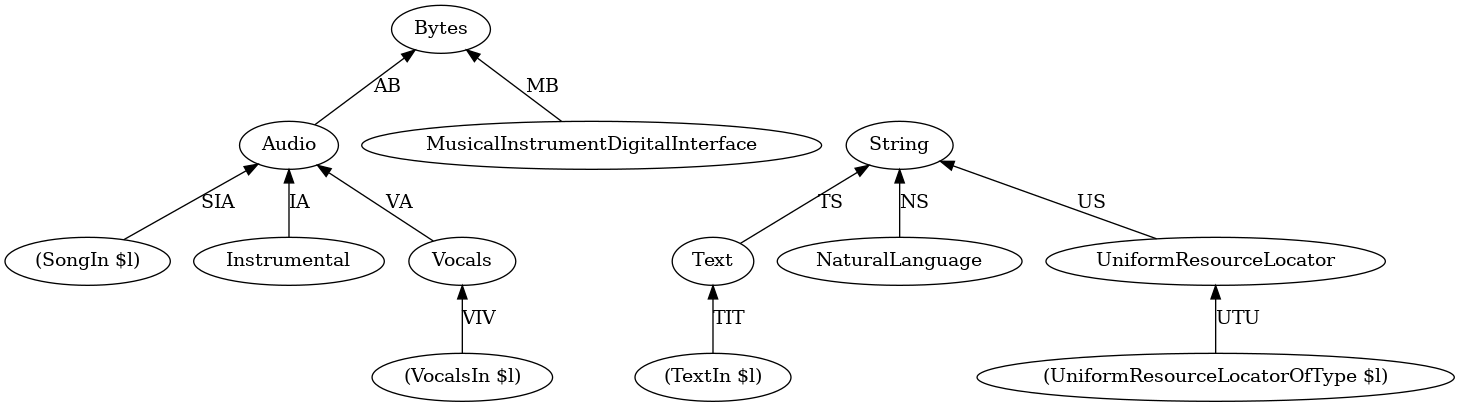
\includegraphics[scale=0.235]{figs/ontology.png}
  \caption{Graphical representation of the miniature ontology
    mentioned earlier.  The nodes represent the types.  The edges
    represent the subtyping relationships, for instance Audio is
    subtype of Bytes is represented by an arrow pointing to Bytes.
    The labels on the edges correspond to the names of axioms encoding
    the subtyping relationships.}
  \label{fig:onto}
\end{figure}
One may observe that in this ontology all types directly or indirectly
derive from primary types such as \mintinline{scheme}{String} and
\mintinline{scheme}{Bytes}.  These primary types comes Protobuf.  What
this means is that, if for instance an AI service outputs data of type
\mintinline{scheme}{Text} to be received by a service that inputs data
of type \mintinline{scheme}{String}, the type coercion may not need to
take place at run-time.  Type coercion is, most of the time, only here
to make sure the AI service composition is consistent with its AI
service specifications.  One may also observe that some types are
parameterized, such as \mintinline{scheme}{(TextIn $l)}, which
represents a text in a certain language \mintinline{scheme}{$l}.
Having parameterized types in the ontology will especially turn out to
be useful while reasoning about dependent types.

Given this ontology we can replace the Protobuf types by semantically
richer types.  Let us consider for instance the
\mintinline{scheme}{naint.machine-translation.MkInput} constructor of
\mintinline{scheme}{naint.machine-translation.Input} mentioned in
Section~\ref{sec:csnmp} and recalled below
\begin{minted}{scheme}
;; Define naint.machine-translation.Input constructor
(: naint.machine-translation.MkInput
   (-> String ; source_lang
       (-> String ; target_lang
           (-> String ; sentences_url
               naint.machine-translation.Input))))
\end{minted}
One can replace the first two occurrences of
\mintinline{scheme}{String} by \mintinline{scheme}{NaturalLanguage}
and the last occurrence of \mintinline{scheme}{String} by
\mintinline{scheme}{(UniformResourceLocatorOfType $t)} or even better
by \mintinline{scheme}{(UniformResourceLocatorOfType Text)} since we
know that this service translates text to text.  But we can do even
better than that and replace it by
\mintinline{scheme}{(UniformResourceLocatorOfType (TextIn $l))} since
we are given the source language as first argument.  The question is
how to specify the source language, for now being just represented as
free variable, \mintinline{scheme}{$l}.  This is where dependent types
shine.  To see how let us rewrite the entire constructor as follows
\begin{minted}{scheme}
;; Define naint.machine-translation.Input constructor with
;; dependent types
(: naint.machine-translation.MkInput
   (-> (: $src-lang NaturalLanguage)
       (-> (: $dst-lang NaturalLanguage)
           (-> (UniformResourceLocatorOfType (TextIn $src-lang))
               (naint.machine-translation.Input $src-lang
                                                $dst-lang)))))
\end{minted}
The variable \mintinline{scheme}{$l} has been replaced by
\mintinline{scheme}{$src-lang}, the inhabitant of the first argument
of \mintinline{scheme}{naint.machine-translation.MkInput}, the source
language of the translation, et voila!  It allows us to express that
the third argument is a type that \emph{depends} on the value of the
first argument.  Also, it goes without saying that replacing
\mintinline{scheme}{String} by a type denoting a location to a datum,
a URL, as opposed to the datum itself allows to catch at
type-checking-time an error that would likely have otherwise occurred
at run-time.  Indeed, it is easy to make the mistake of plugging in
input of the translator a service that directly outputs a text as
opposed to a URL pointing to the text to translate.  Finally, one
should note that the
\mintinline{scheme}{naint.machine-translation.Input} type has been
replaced by a parameterized type, taking the source and destination
languages as parameters, which is needed not to lose that information
downstream.  Likewise the
\mintinline{scheme}{naint.machine-translation.Output} type has been
replaced by a parameterized type simply taking the destination
language as parameter as the information about the source language is
no longer needed.  The
\mintinline{scheme}{naint.machine-translation.translate} method thus
looks like
\begin{minted}{scheme}
;; Define naint.machine-translation.translate service method
(: naint.machine-translation.translate
   (-> (naint.machine-translation.Input $src-lang $dst-lang)
       (naint.machine-translation.Output $dst-lang)))
\end{minted}
In the AI service composition experiments described in
Chapter~\ref{chap:xpaicompo}, the above has been further simplified by
embedding the input and output constructors directly in the arguments
of the \mintinline{scheme}{naint.machine-translation.translate}
method, resulting into the following type signature
\begin{small}
\begin{minted}{scheme}
;; Define naint.machine-translation.translate service method
(: naint.machine-translation.translate
   (-> (: $src-lang NaturalLanguage)
       (: $dst-lang NaturalLanguage)
       (-> (: $url (UniformResourceLocatorOfType (TextIn $src-lang)))
           (TextIn $dst-lang))))
\end{minted}
\end{small}
One may also notice that the fully curried representation has been
replaced by some hybrid curried-uncurried one.  Indeed the first two
arguments, the source and destination languages, are uncurried while
the last one, the URL pointing to the text to translate, is curried.
This is because we have found that it mitigate the combinatorial
explosion to cleaning separate parameters (like the source and
destination languages) and data to be processed (like the text to be
translated).

It all looks good and well, but there is one elephant in the Section.
How to automate such type enrichment process?  How to go from a given
Protobuf specification to a MeTTa specification?  How to choose the
right semantically rich type in the ontology as a substitute for a
semantically poor type in the Protobuf specification.  And finally,
how to come up with the ontology in the first place?  As valid as
these questions are, they are left aside in this technical report, but
will undoubtedly resurface in the future when their time is right.

\chapter{Experimenting with AI Service Composition in MeTTa}
\label{chap:xpaicompo}
We have written a few prototypes in MeTTa, all based on the backward
chainers presented in Chapter~\ref{chap:chainers}, to synthesize AI
service compositions.  In this chapter we will describe the various
experiments we have conducted with some benchmarks and a few lessons
that we have learned along the way.

\section{Experimental Setup}
\label{sec:xpsetup}

\subsection{AI Service Compositions}
After perusing the SingularityNET marketplace to find meaningful AI
service compositions to attempt to synthesize them, we have retained
two compositions:
\begin{enumerate}
\item \textbf{Speech Emotion Recognition}, obtained by sequentially
  combining two services, \texttt{speech2text-en} and
  \texttt{text-emotions}, provided by the NAINT organization,
  represented by the following flowchart-like graph:
  \begin{center}
    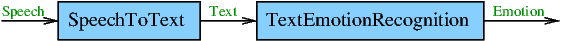
\includegraphics[scale=0.55]{figs/SimpleSpeechEmotionRecognition.png}
  \end{center}
  The graph says it all, speech is turned into text, then emotion is
  detected from this text.  One could easily envision a variation
  involving a parallel composition of another service that can detect
  emotion in speech directly, more focused and voice expression than
  semantics, but in this report we purposely leave it at that, a
  simple composition involving two services.
\item \textbf{English to Chinese Song Translation}, obtained to by
  combining the following services, \texttt{sound-spleeter} and
  \texttt{speech-recognition} from SingularityNET,
  \texttt{machine-translation} and \texttt{midi2voice-zh} from NAINT.
  In addition we have added an extra service, \texttt{tomidi}, to
  convert audio to MIDI.  This service is not present on the
  SingularityNET marketplace so we had to handwrite it in MeTTa rather
  than obtain it from the crawler described in
  Chapter~\ref{chap:marketplace}.  We also had to add a micro service
  to mix two audio signals, \texttt{mixer}, also not present in the
  SingularityNET marketplace.  The flowchart-like graph below
  represents the composition we wish to synthesize.
  \begin{center}
    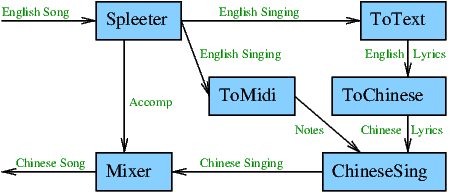
\includegraphics[scale=0.6]{figs/EnglishToChineseSong.png}
  \end{center}
  The flow of information is a bit more complicated here.  An audio
  signal encoding an English song comes in, it is split into two audio
  signals, one for the instrumental and the other one for the vocals.
  The instrumental, \texttt{Accomp} in the graph, goes straight to the
  mixer.  The vocals on the other hand is further duplicated into two
  signals, one converted into text, the lyrics, then translated to
  Chinese, the other converted into MIDI, the melody.  Both the
  Chinese lyrics and the melody then join into the Chinese singing
  service to produce Chinese vocals.  Finally the instrumental and the
  Chinese vocals get mixed to produce the Chinese song.  Making this
  work in practice is actually more involved than just plugging these
  services as described and requires syncing the Chinese vocals and
  the instrumental.  But regardless of the run-time result, what is of
  interest to us here is whether the AI-DSL is able to synthesize such
  AI service composition.
\item Additionally, our experiments contains a third AI service
  composition which is a scaled down version of the English to Chinese
  Song Translation shown below, defined to create an intermediary
  level of difficulty in synthesis between the Speech Emotion
  Recognition composition and the English to Chinese Song Translation
  composition.
  \begin{center}
    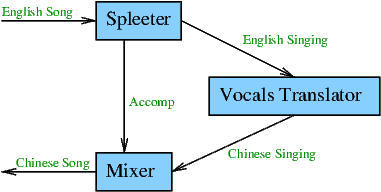
\includegraphics[scale=0.6]{figs/EnglishToChineseSongScaledDown.png}
  \end{center}
  In this composition the translation from English text to Chinese
  text, melody recognition and Chinese singing generation has been
  replaced by a single service, \textbf{Vocals Translator}.  This
  service does not exists on the SingularityNET marketplace thus was
  handcoded.
\end{enumerate}
\subsection{Search Space}
For each AI service composition, the search space is limited to the
services involved.  Meaning we do not dump the entire SingularityNET
marketplace into the knowledge based of the chainer.  So for instance
for the Speech Emotion Recognition composition, only two services are
described.  This involves more than two axioms because services have
data constructors and access functions.  But this nonetheless
dramatically reduces the search space.  As we will see though, even
with that simplification, in the absence of any pruning, the search
can already easily become intractable.  Much of the lessons learned
during these experiments have to do with pruning the search.
\subsection{Backward Chaining Variations}
In order to cope with combinatorial explosion we had to experiment
with numerous variations of the backward chainer, such as
\begin{itemize}
\item Lambda abstraction, which is a powerful way to produce
  compositions with arbitrary complex information flow.
\item Combinatory logic, which is also a powerful way to achieve
  arbitrary complex information flow.
\end{itemize}
Combinatorial power also comes with combinatorial explosion, thus to
prune the search we have experimented with
\begin{itemize}
\item Limiting the flow of information to data, as opposed to
  functions.  Meaning that on the wires on the composition only data
  can transit, not functions.
\item Adding reduction rules to avoid synthesizing syntactically
  different yet semantically identical candidates (similarly to how
  MOSES~\cite{TODO} uses reduction as pruning technique).
\item Uncurrify services and combinators.  This has the interesting
  effect of pruning the search by avoiding combining the services in
  weird, higher order ways, quite similar to limiting the information
  flow to data, but even stronger.
\end{itemize}
In the end we have found that using reduction rules and some well
selected uncurried combinators enabled efficient synthesis of AI
service compositions, for our limited setting anyway.

\chapter{Conclusion}
\section{Future Developments}
\begin{enumerate}
\item Manage resources, financial, computational.
\item Reason about uncertainty of outcomes (probability of failing,
  average accuracy of the results, etc).
\item Use infer grained language that captures not just functional
  semantics but also run-time behavior.
\item How to build the ontology and enrich Protobuf specifications to
  leverage such ontology.
\end{enumerate}

\section{Acknowledgments}
Thanks to Matt Ikle and Khellar Crawford for our numerous discussions.
Thanks to Remy Clarke for mentioning APL and BQN.  Thanks to Douglas
Miles for making MeTTaLog which has been tremendously helpful for
running some experiments.

\appendix
\chapter{DOT Format Conversion}
\label{apdx:dot}

\bibliographystyle{splncs04} \bibliography{local}

\end{document}
